\clearpage
\newpage
%********************************************************************************
\section{MCMC Samples from different Calibration Schemes}\label{app:mcmc_samples}
%********************************************************************************

% Marginals of the joint posterior samples, Calibration with TC Output only
\rotatebox{90}{\begin{minipage}{0.85\textheight}
    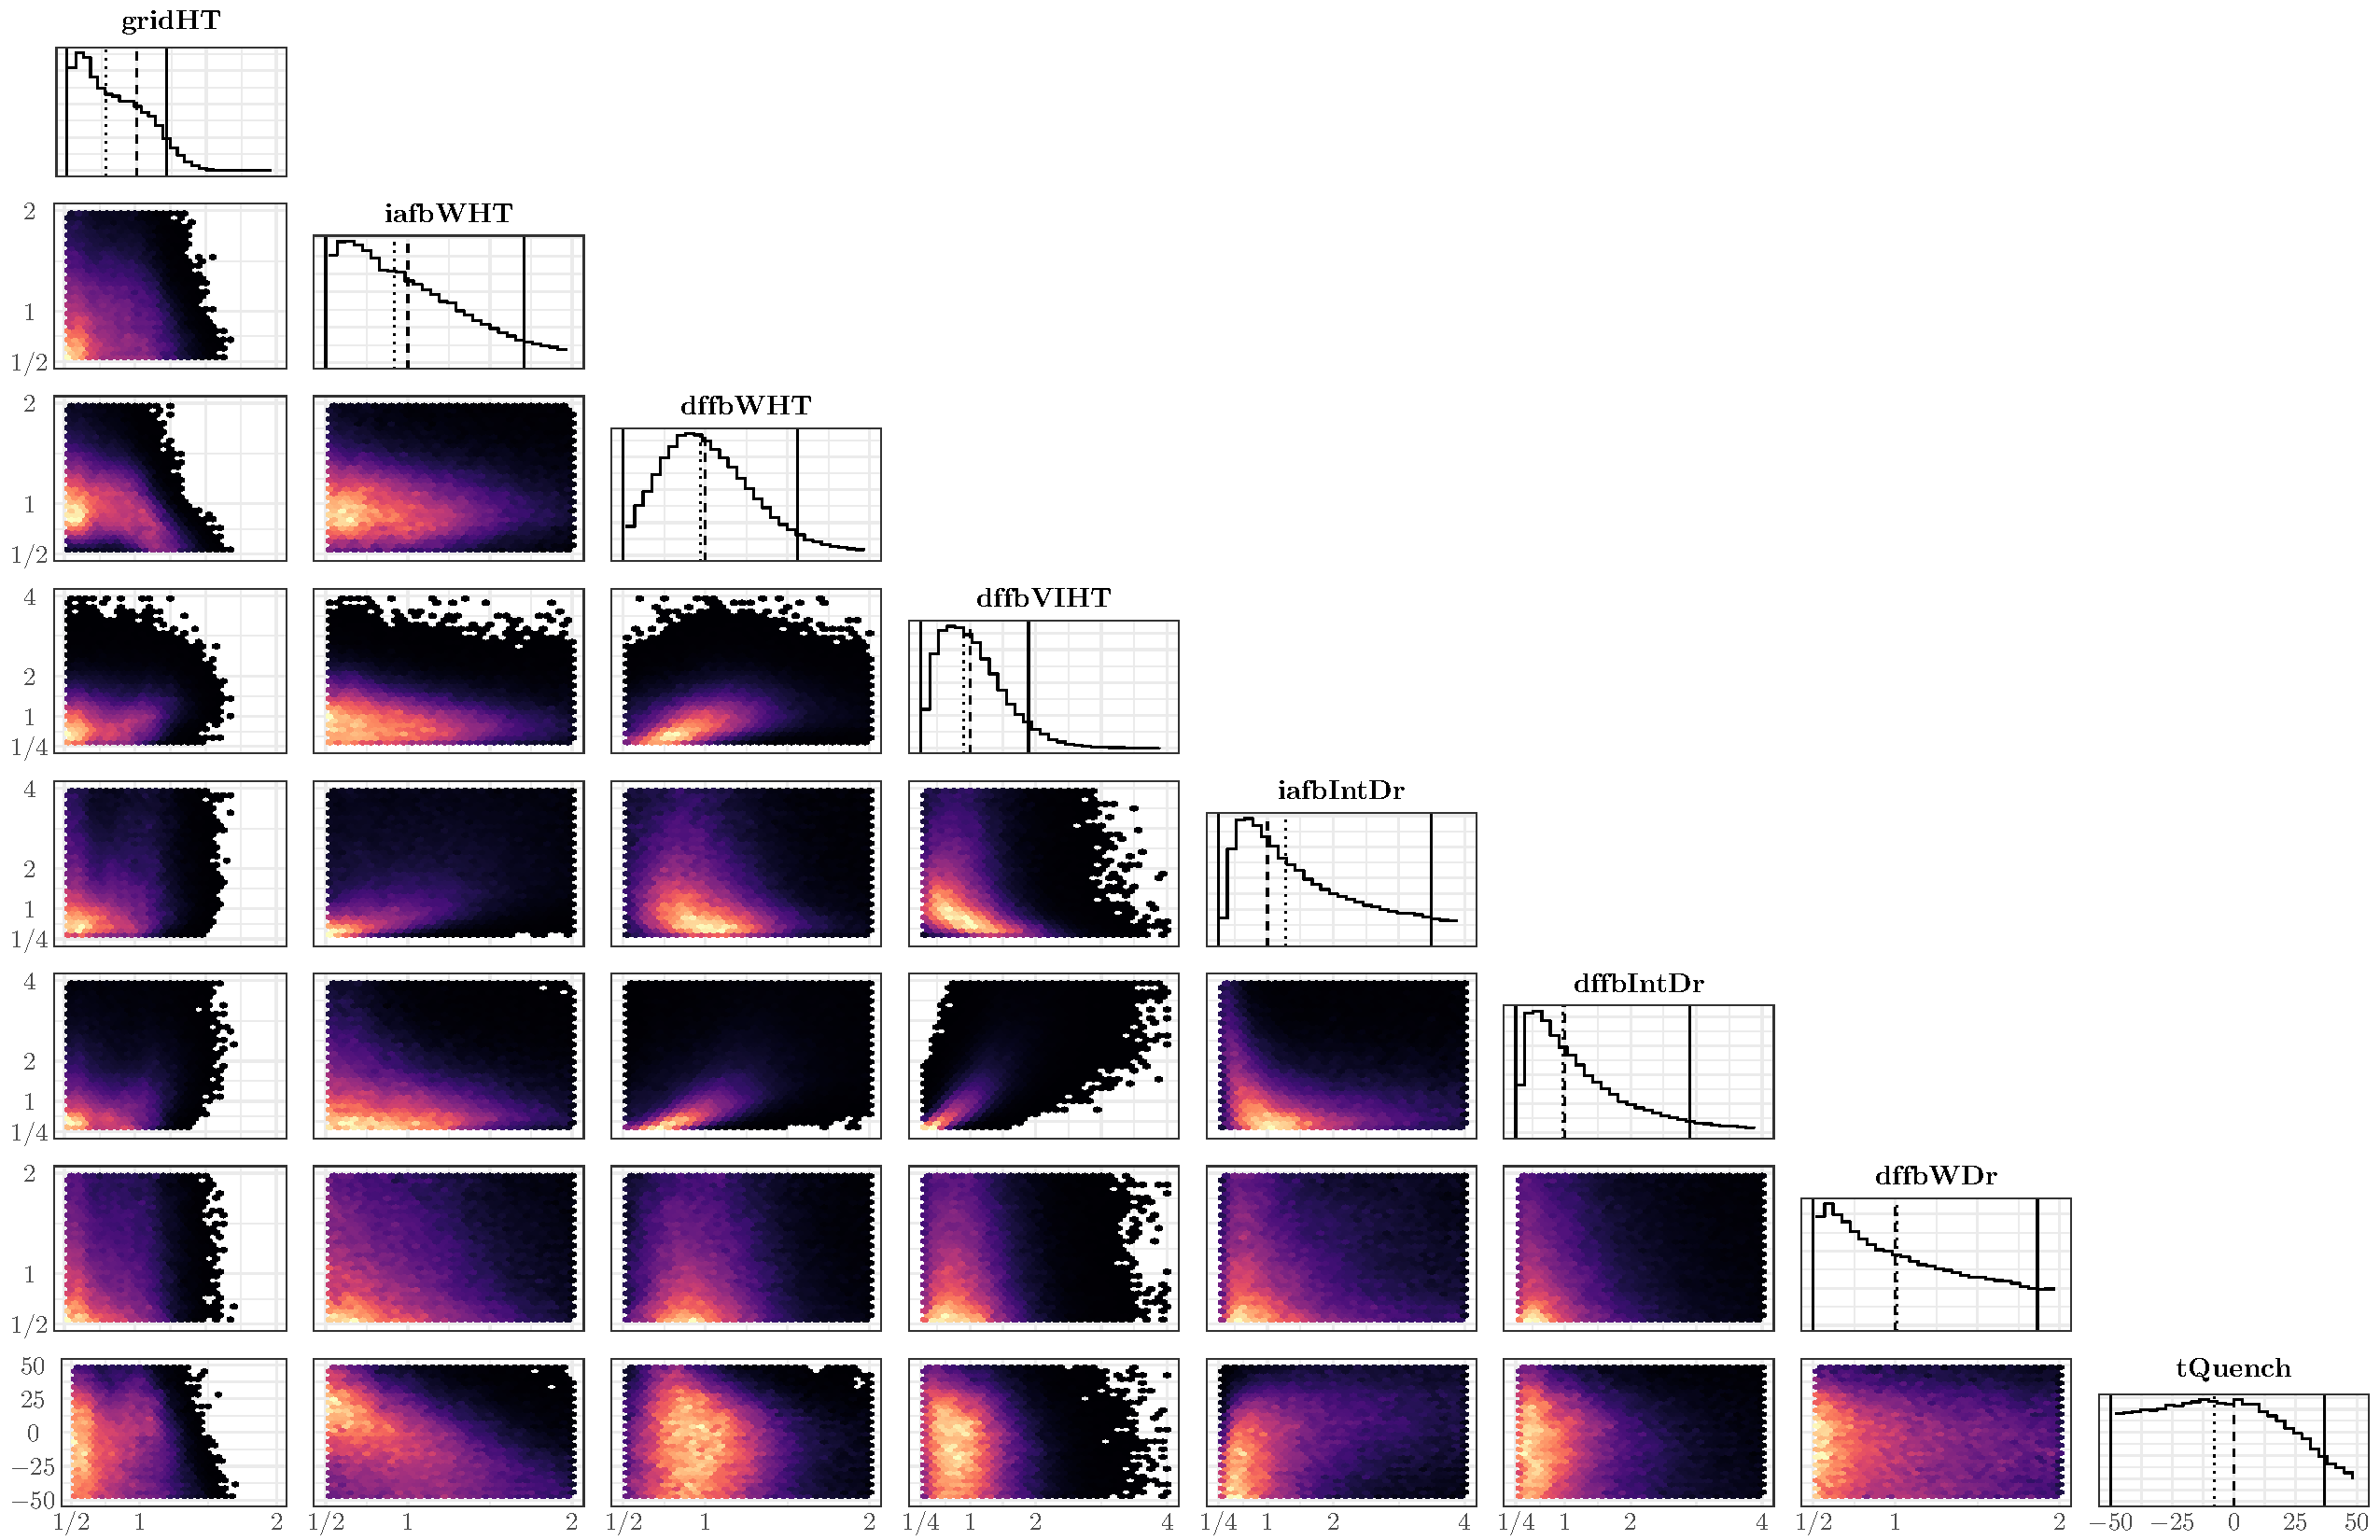
\includegraphics[width=0.9\textwidth]{../figures/chapter5/figures/plotEnsTCDiscCentered}
		\captionof{figure}[Univariate and bivariate marginals of the posterior samples for each of the $8$ model parameters. Calibration with respect to the cladding temperature output ($TC$) and with model bias term.]{Univariate and bivariate marginals of the posterior samples for each of the $8$ model parameters. Solid lines, dashed, and dotted lines indicate the $95\%$ \glspl[hyper=false]{hpdi}, the nominal parameter values, and the posterior median parameter values. Calibration with respect to the cladding temperature output ($TC$) and with model bias term.}
    \label{fig:ch5_plot_ens_tc_disc_centered}
\end{minipage}}

% Marginals of the joint posterior samples, Calibration with DP Output only
\clearpage
\begin{sidewaysfigure}
	\centering
	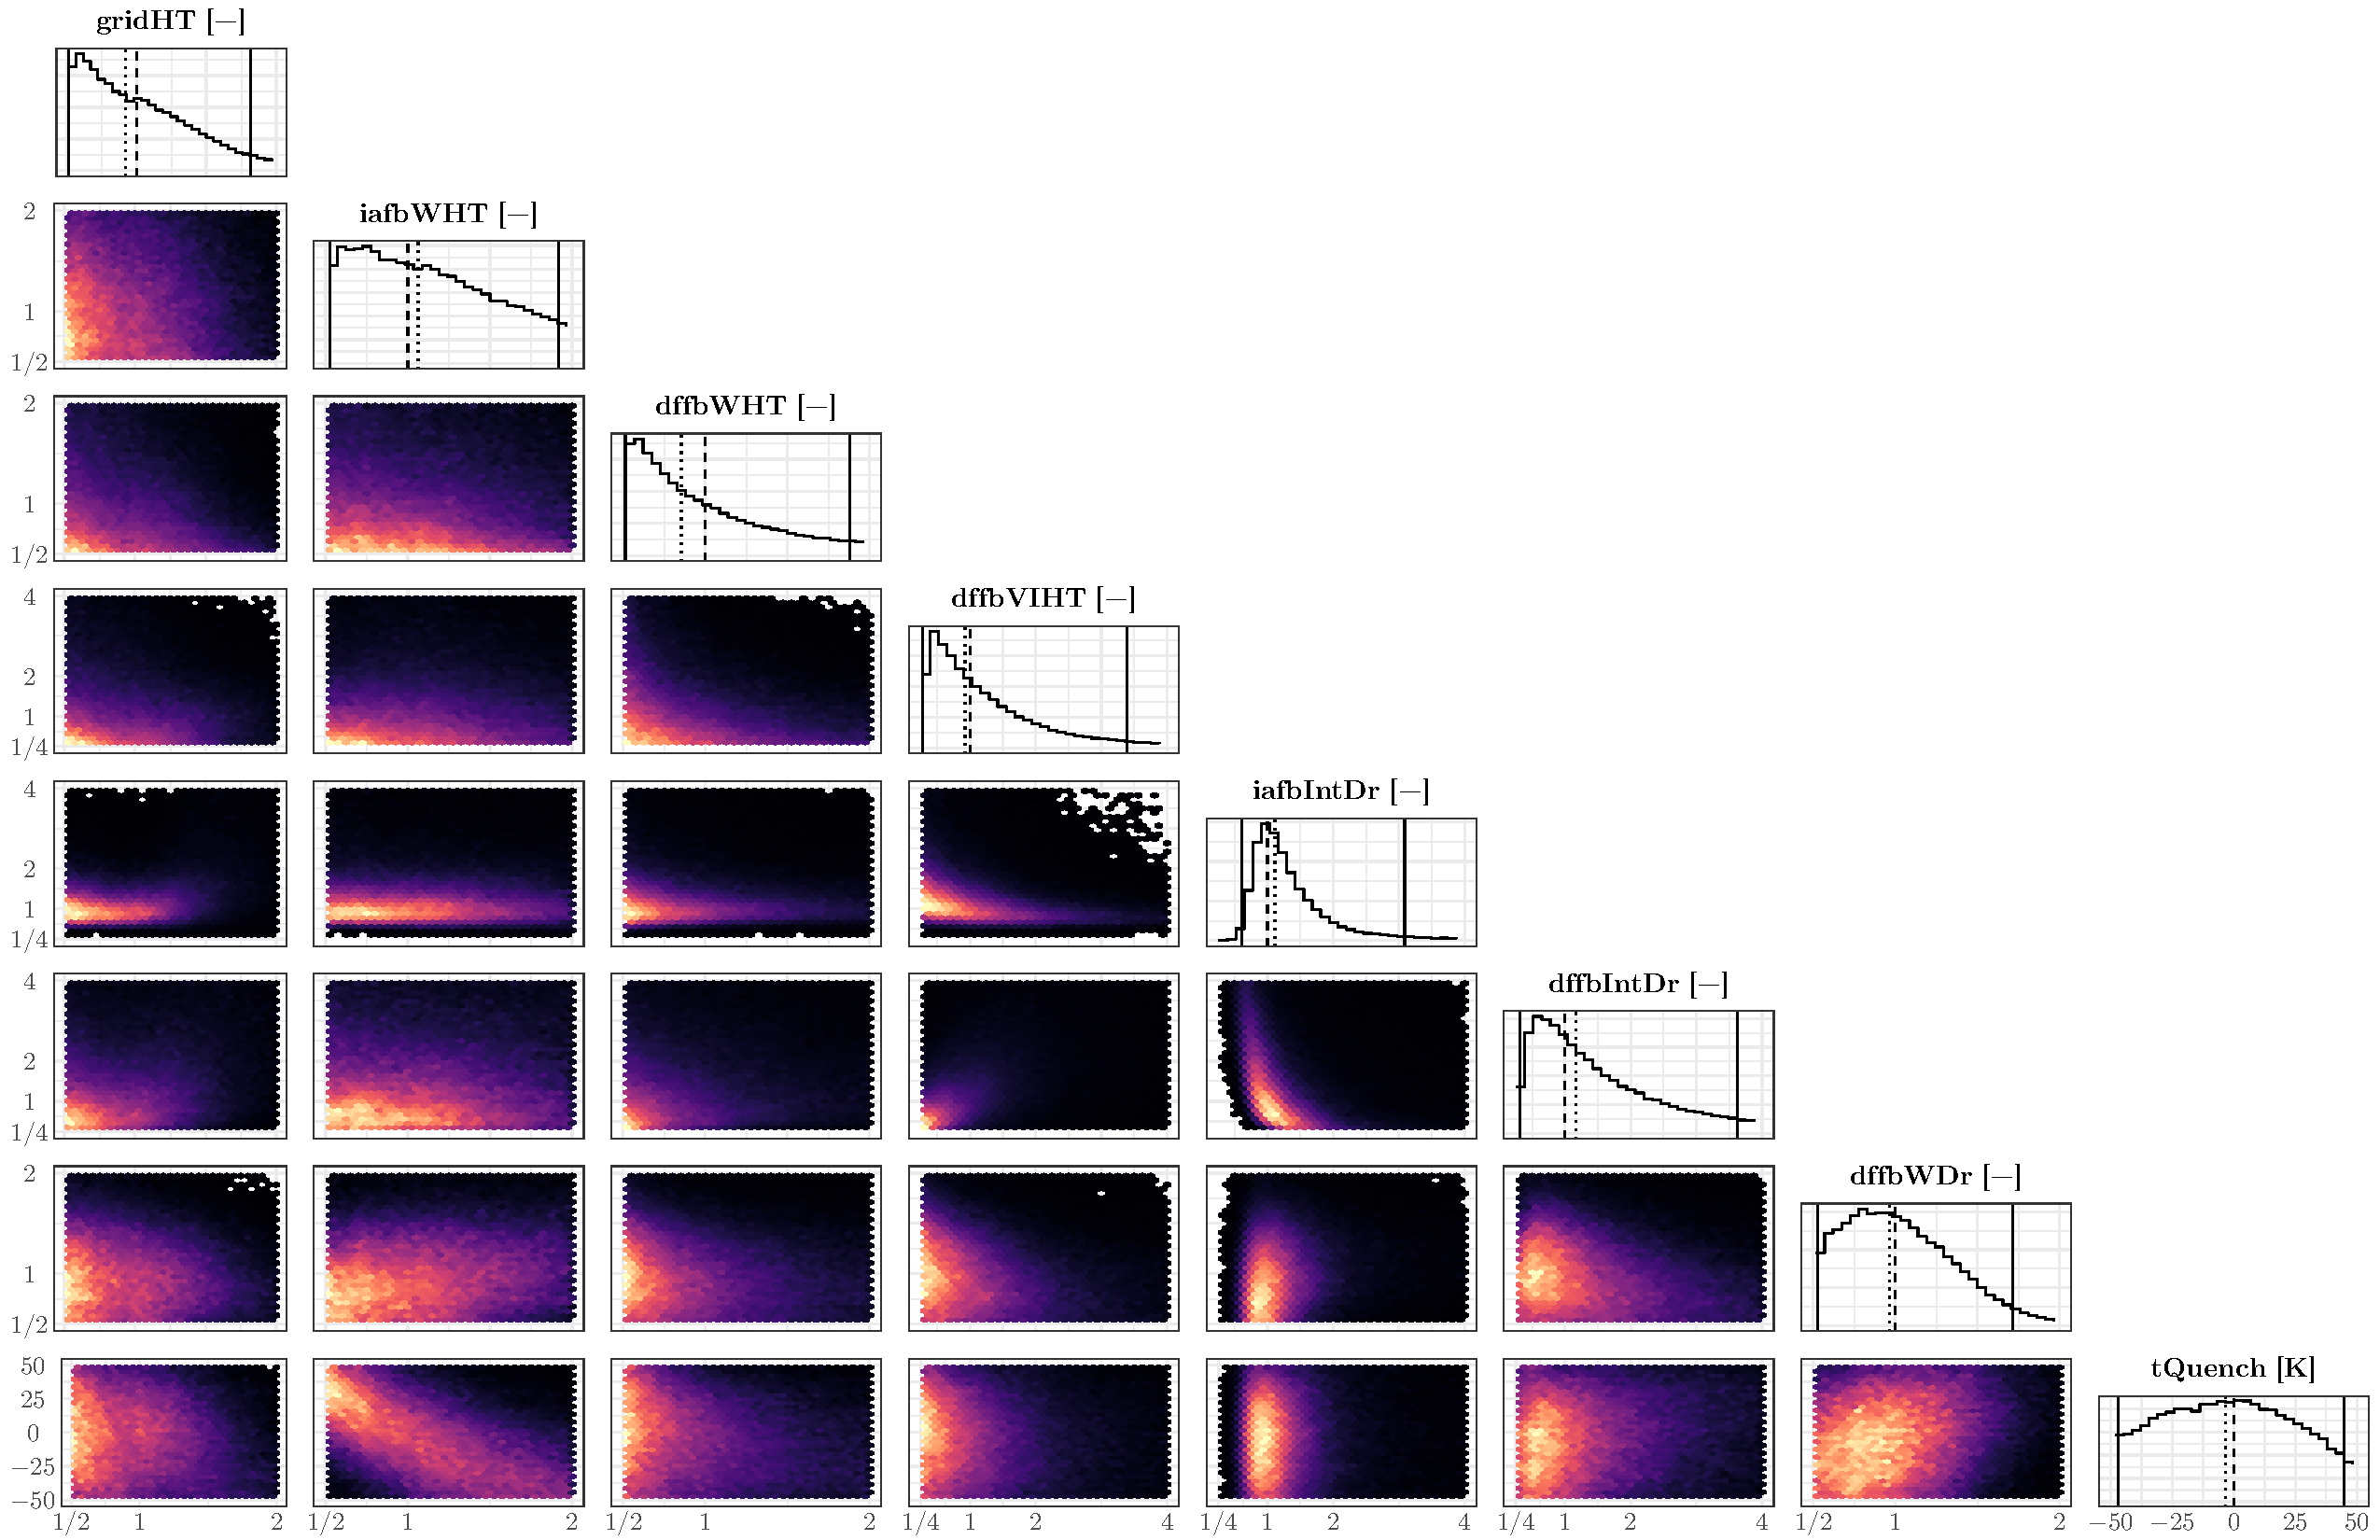
\includegraphics[width=0.85\textwidth]{../figures/chapter5/figures/plotEnsDPDiscCentered}
		\captionof{figure}[Univariate and bivariate marginals of the posterior samples for each of the $8$ model parameters. Calibration with respect to the pressure drop output ($DP$) and with model bias term.]{Univariate and bivariate marginals of the posterior samples for each of the $8$ model parameters. Solid lines, dashed, and dotted lines indicate the $95\%$ \glspl[hyper=false]{hpdi}, the nominal parameter values, and the posterior median parameter values. Calibration with respect to the pressure drop output ($DP$) and with model bias term.}
	\label{fig:ch5_plot_ens_dp_disc_centered}
\end{sidewaysfigure}

% Marginals of the joint posterior samples, Calibration with CO Output only
\clearpage
\begin{sidewaysfigure}
	\centering
	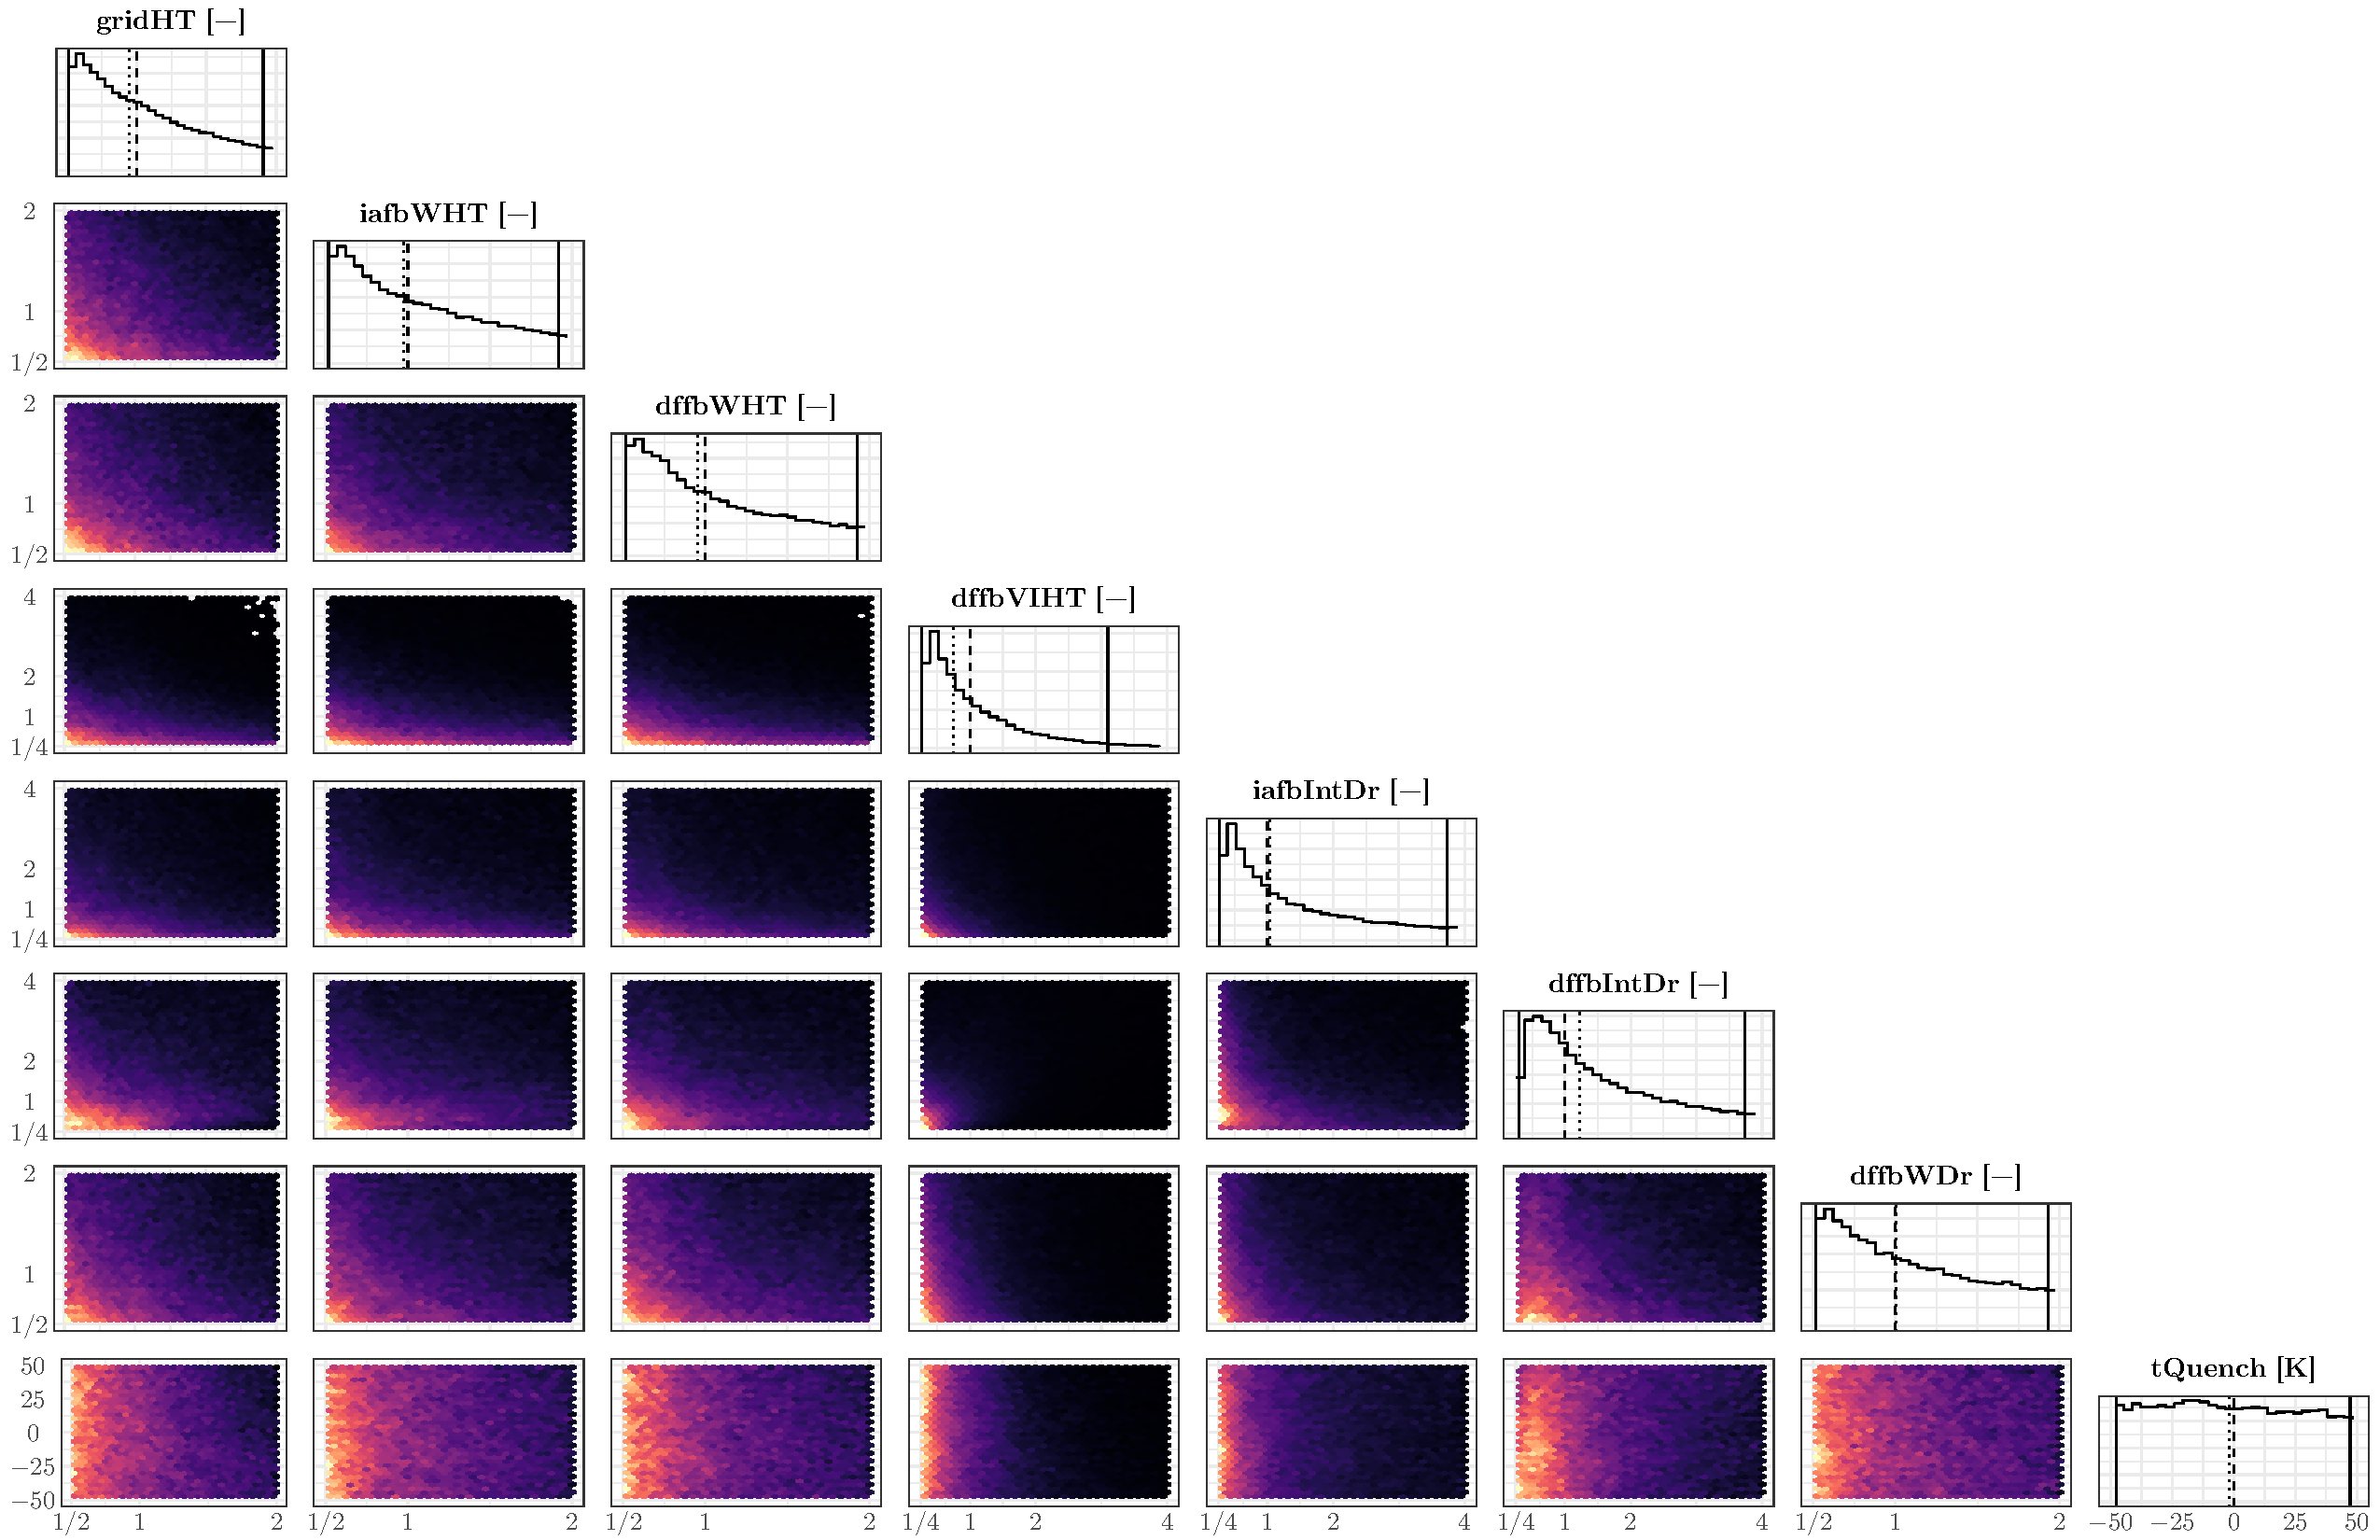
\includegraphics[width=0.85\textwidth]{../figures/chapter5/figures/plotEnsCODiscCentered}
		\captionof{figure}[Univariate and bivariate marginals of the posterior samples for each of the $8$ model parameters. Calibration with respect to the liquid carryover output ($CO$) and with model bias term.]{Univariate and bivariate marginals of the posterior samples for each of the $8$ model parameters. Solid lines, dashed, and dotted lines indicate the $95\%$ \glspl[hyper=false]{hpdi}, the nominal parameter values, and the posterior median parameter values. Calibration with respect to the liquid carryover output ($CO$) and with model bias term.}
	\label{fig:ch5_plot_ens_co_disc_centered}
\end{sidewaysfigure}

% Marginals of the joint posterior samples, No Param 8
\clearpage
\begin{sidewaysfigure}
	\centering
	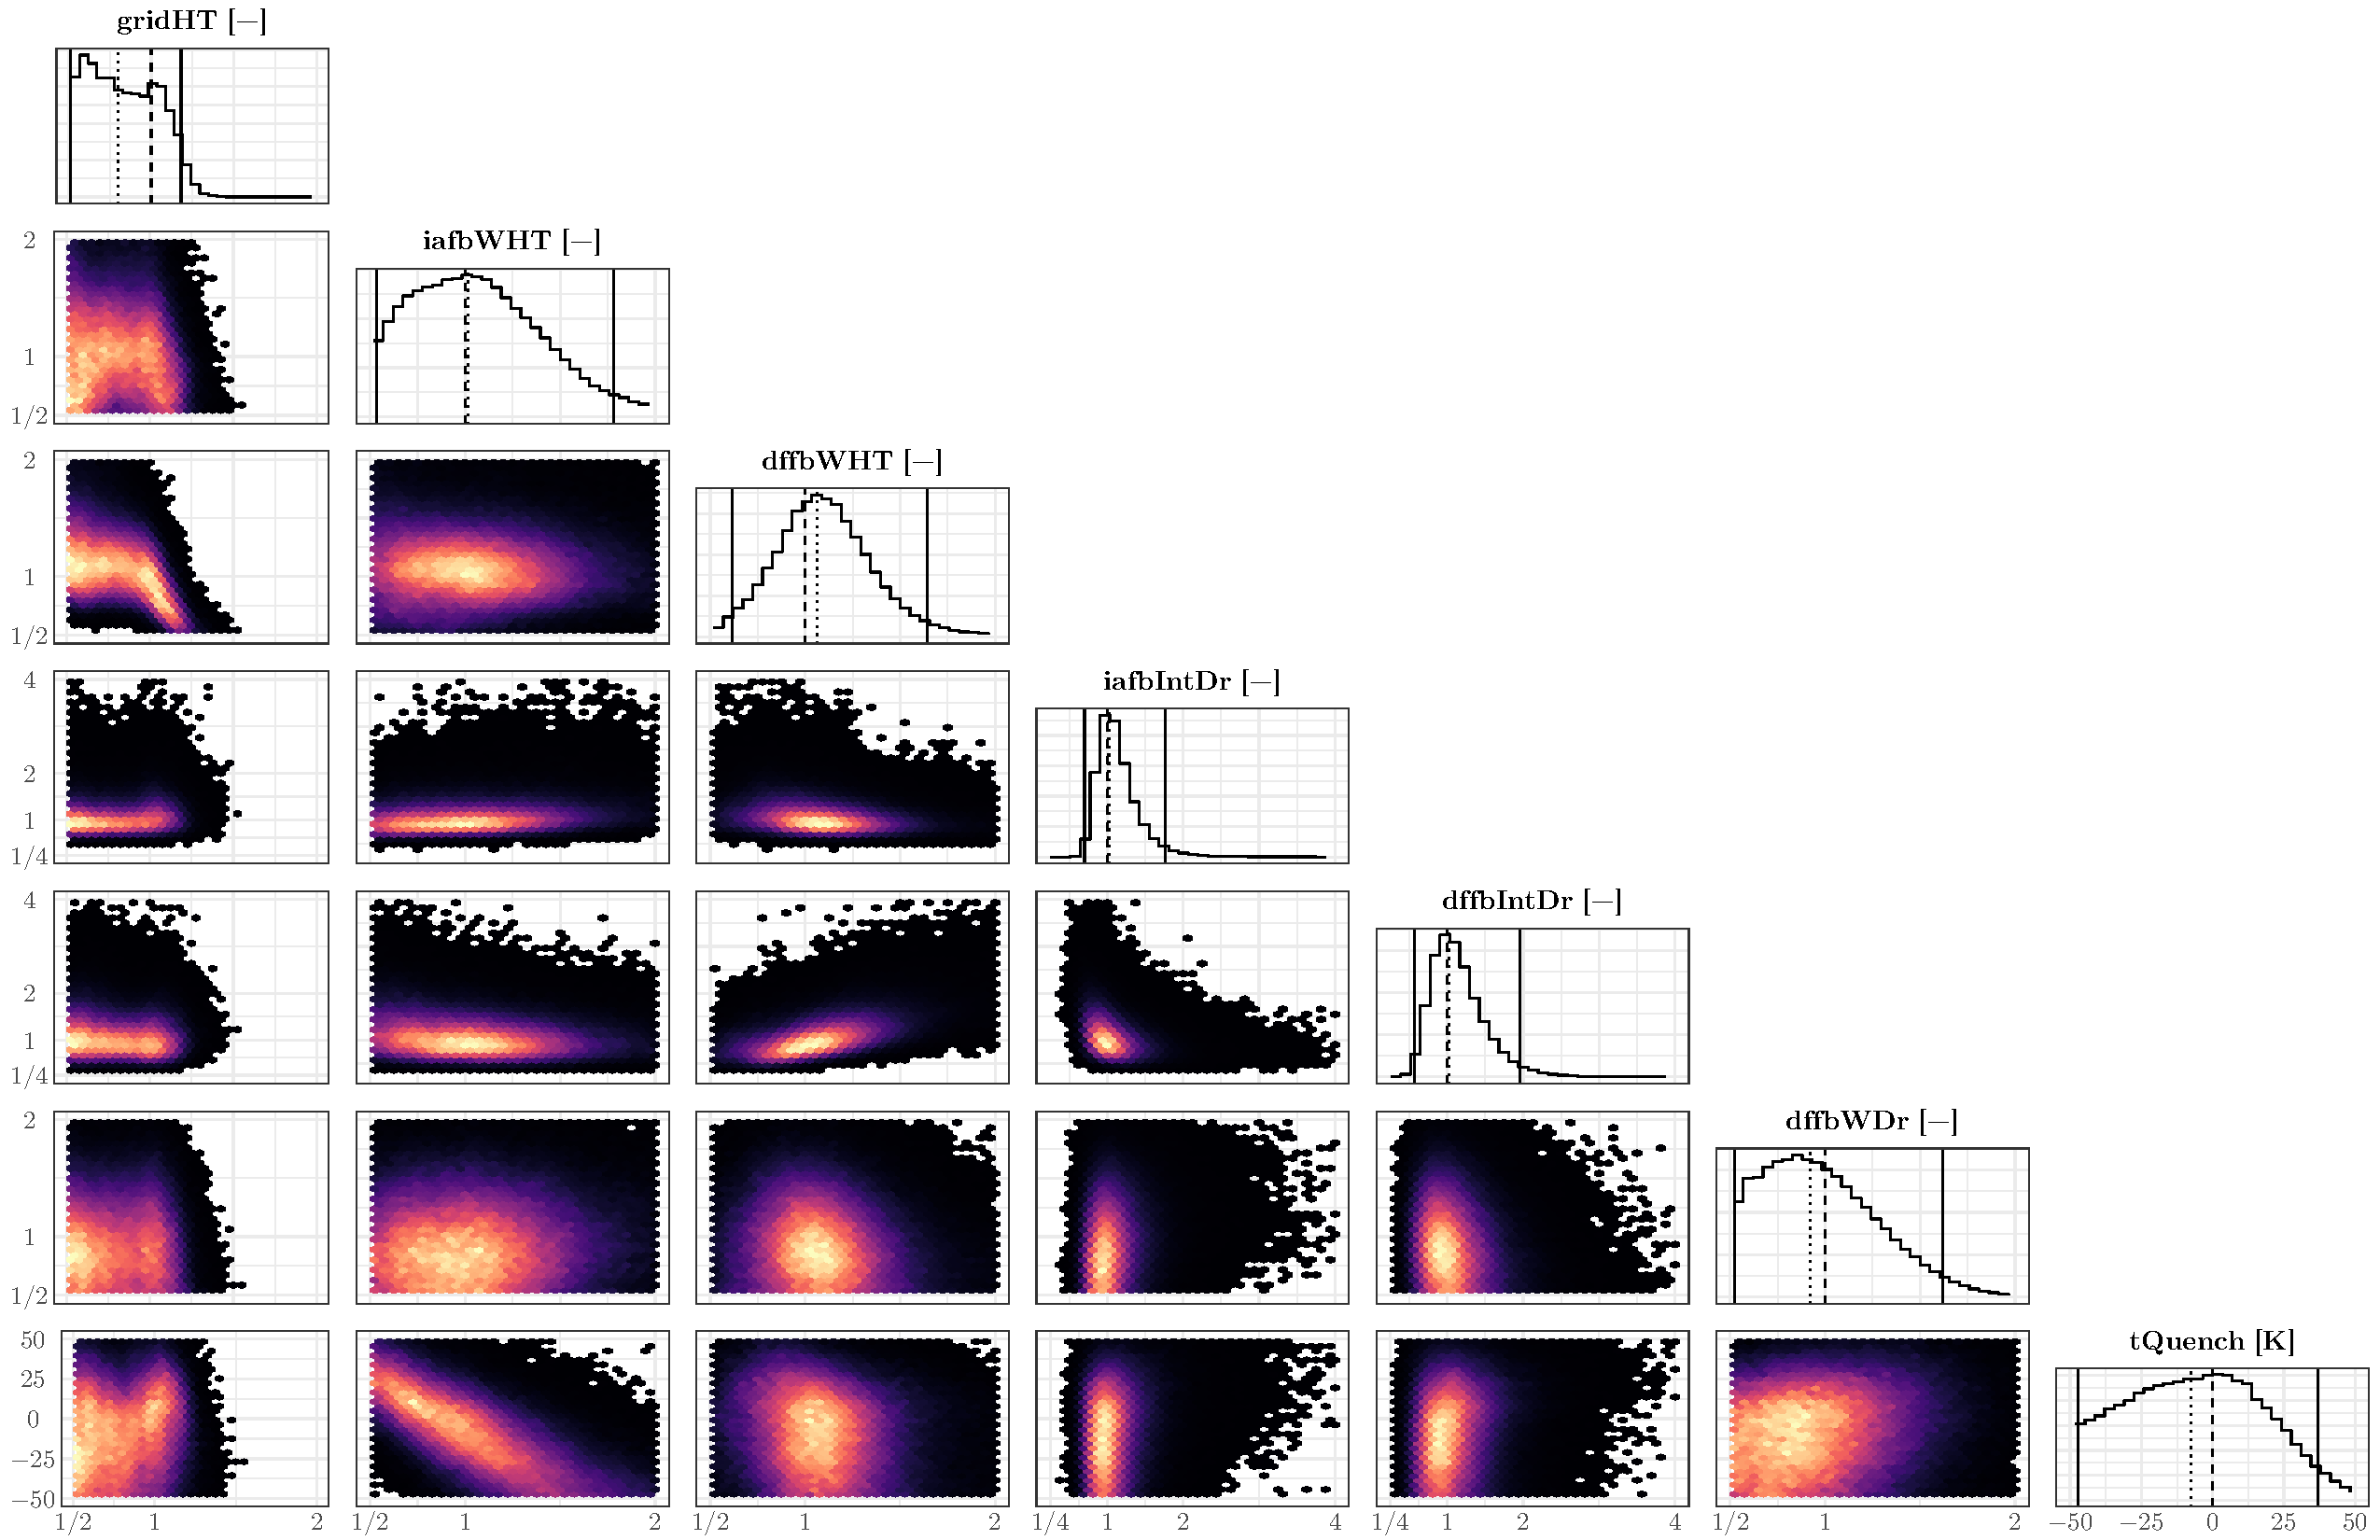
\includegraphics[width=0.85\textwidth]{../figures/chapter5/figures/plotEnsAllDiscCenteredNoParam8}
		\captionof{figure}[Univariate and bivariate marginals of the posterior samples for each of the $7$ model parameters, excluding \texttt{dffbVIHTC} parameter. Calibration with respect to all types of output ($TC$, $DP$, and $CO$) and without model bias term.]{Univariate and bivariate marginals of the posterior samples for each of the $8$ model parameters, excluding \texttt{dffbVIHTC} parameter. Solid lines, dashed, and dotted lines indicate the $95\%$ \glspl[hyper=false]{hpdi}, the nominal parameter values, and the posterior median parameter values. Calibration with respect to all types of output ($TC$, $DP$, and $CO$) and without model bias term.}
	\label{fig:ch5_plot_ens_all_disc_centered_noparam8}
\end{sidewaysfigure}

% Marginals of the joint posterior samples, No Model Bias Term
\clearpage
\begin{sidewaysfigure}
	\centering
	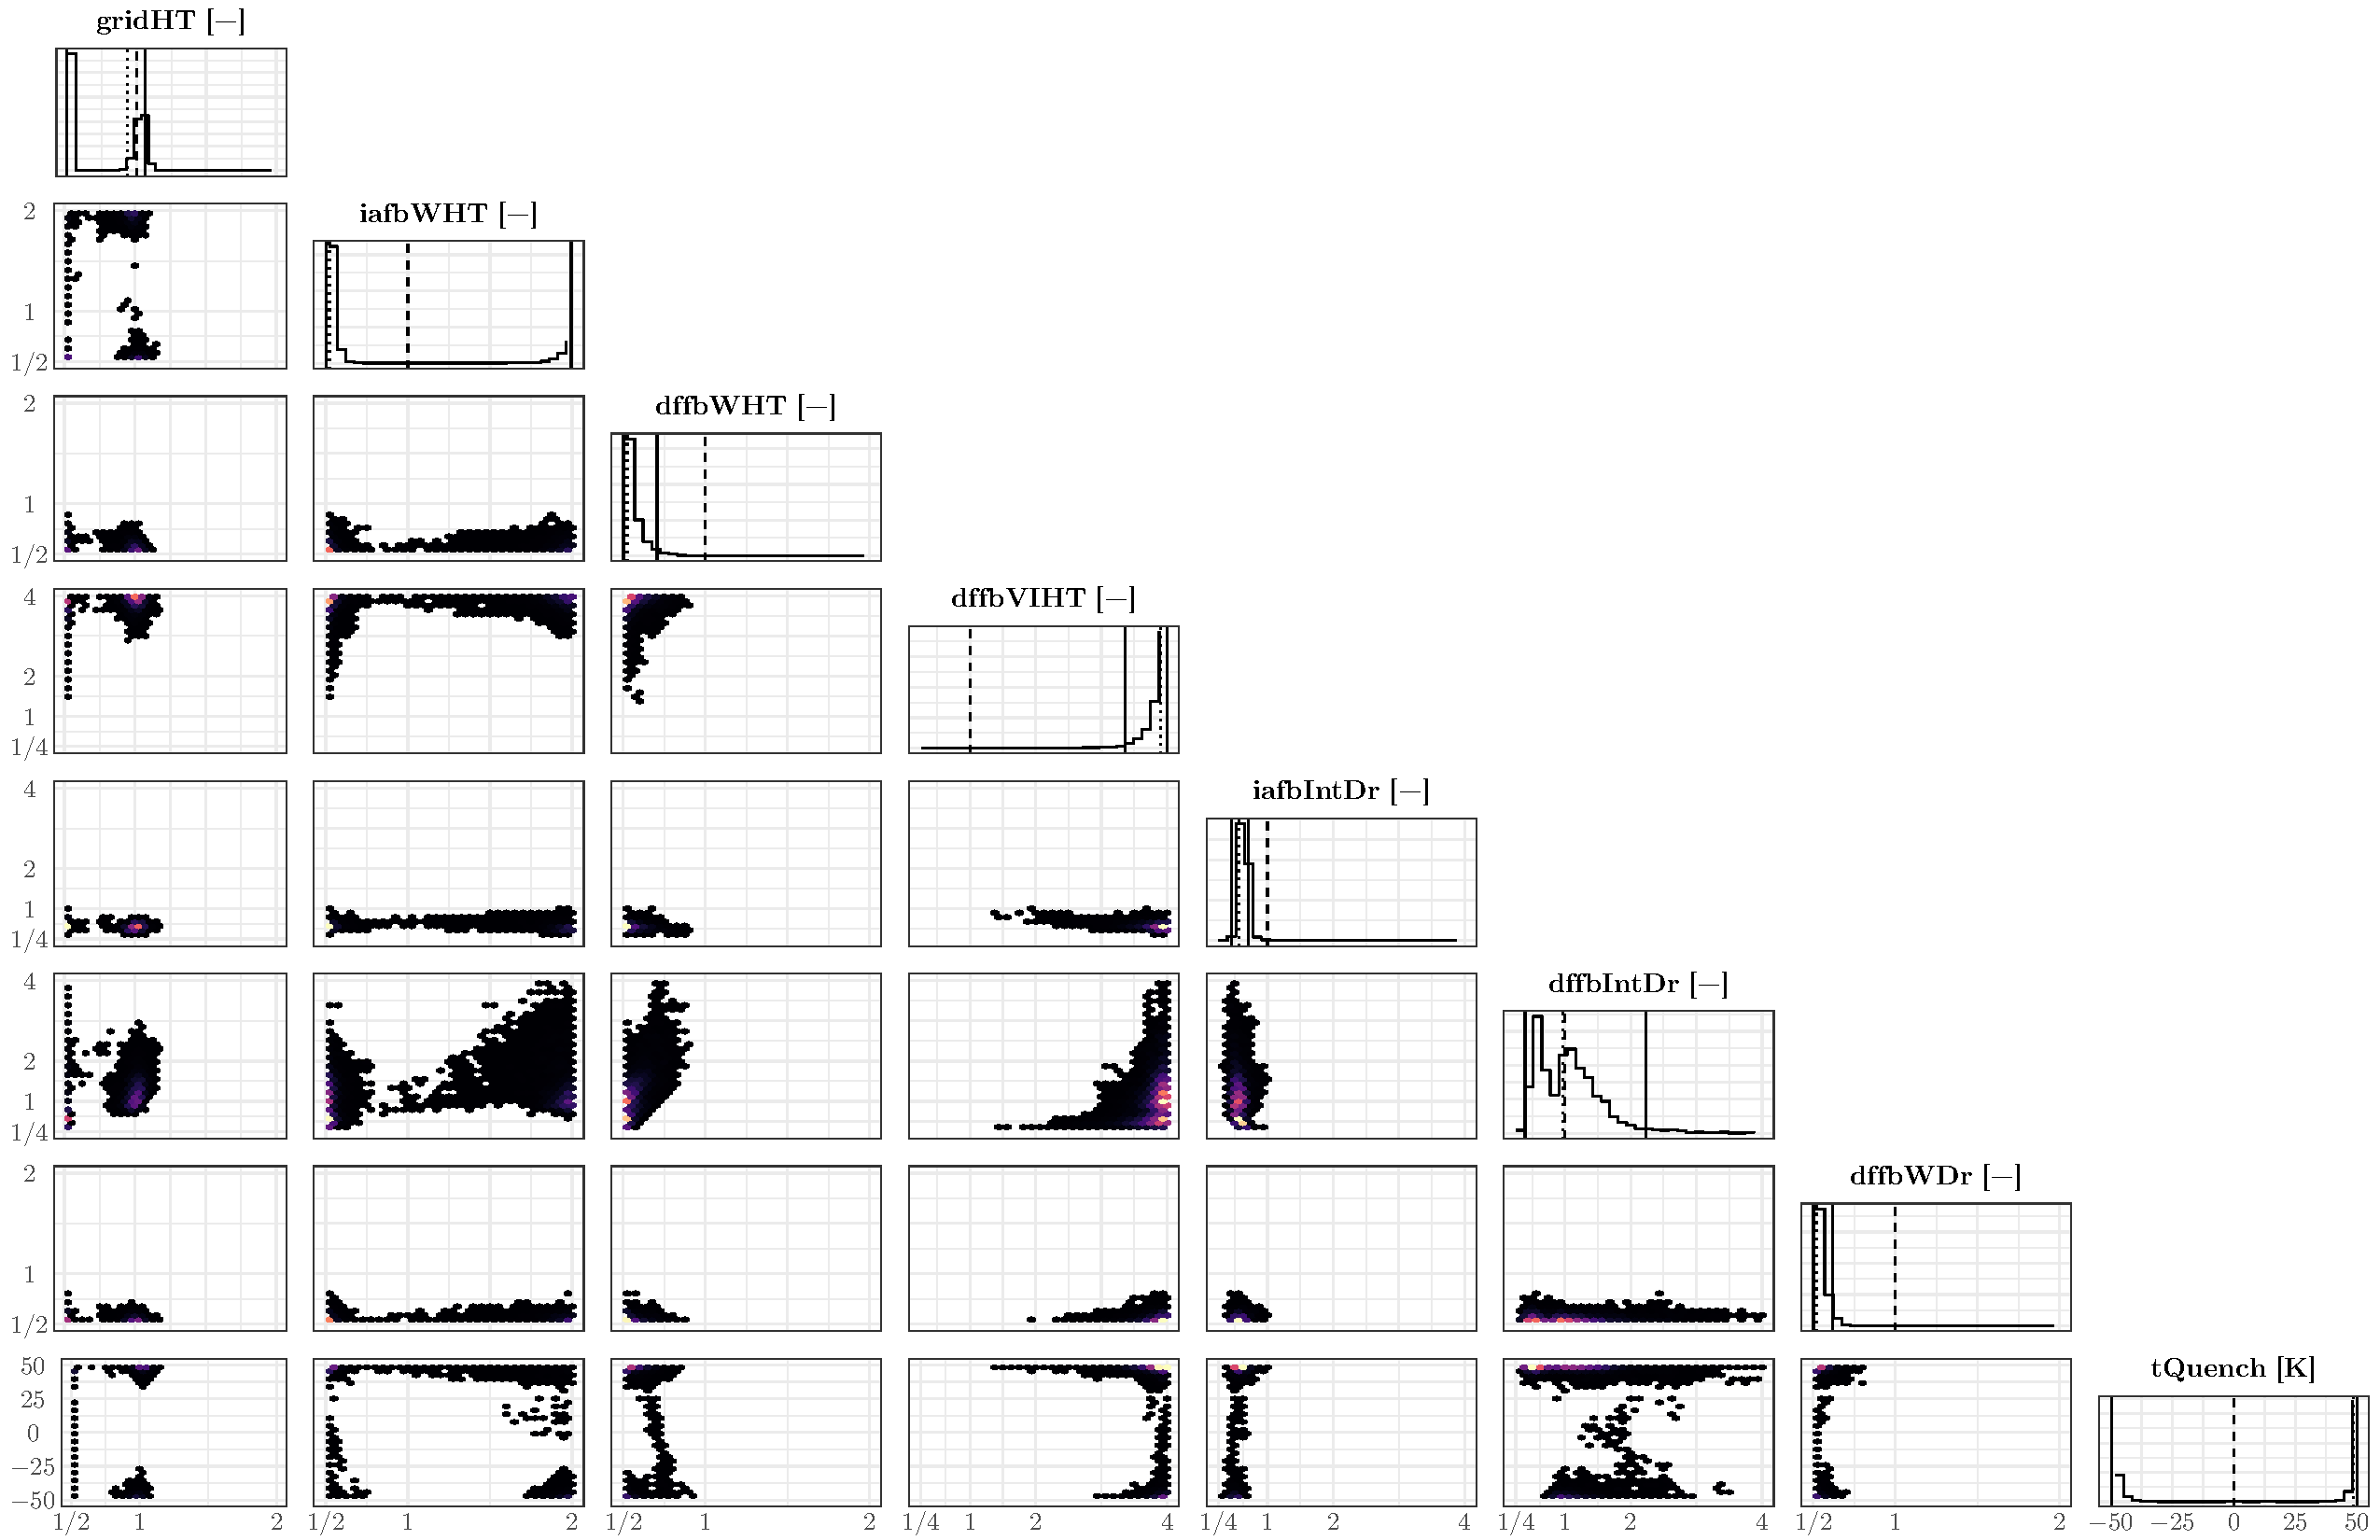
\includegraphics[width=0.85\textwidth]{../figures/chapter5/figures/plotEnsAllNoDiscNoBC}
		\captionof{figure}[Univariate and bivariate marginals of the posterior samples for each of the $8$ model parameters. Calibration with respect to all types of output ($TC$, $DP$, and $CO$) and without model bias term.]{Univariate and bivariate marginals of the posterior samples for each of the $8$ model parameters. Solid lines, dashed, and dotted lines indicate the $95\%$ \glspl[hyper=false]{hpdi}, the nominal parameter values, and the posterior median parameter values. Calibration with respect to all types of output ($TC$, $DP$, and $CO$) and without model bias term.}
	\label{fig:ch5_plot_ens_all_nodisc}
\end{sidewaysfigure}
\clearpage